\documentclass[conference]{IEEEtran}
\IEEEoverridecommandlockouts

\usepackage{cite}
\usepackage{amsmath,amssymb,amsfonts}
\usepackage{amsthm}
\usepackage{algorithm}
\usepackage{algorithmic}
\renewcommand{\algorithmicrequire}{\textbf{Input:}}
\renewcommand{\algorithmicensure}{\textbf{Output:}}
\usepackage{graphicx}
\usepackage{booktabs}
\usepackage{placeins}
\usepackage{microtype}
\linespread{0.97}
\setlength{\textfloatsep}{10pt plus 2pt minus 2pt}
\setlength{\dbltextfloatsep}{10pt plus 2pt minus 2pt}
\usepackage[hidelinks]{hyperref}
\hypersetup{
  pdftitle={ALPS: Admissible Locality and Payload Semantics for Region-Based Parallel Mining},
  pdfauthor={M Mohaiminul Islam}
}

\newtheorem{theorem}{Theorem}
\newtheorem{proposition}{Proposition}
\newtheorem{definition}{Definition}
\newtheorem{corollary}{Corollary}

\begin{document}

\title{$ALPS$: Admissible Locality and Payload Semantics\\
for Region-Based Parallel Mining}

\author{\IEEEauthorblockN{M Mohaiminul Islam}
\IEEEauthorblockA{\textit{Department of Computer Science \& Telecommunication Engineering}\\
\textit{}\\
}}

\maketitle

\begin{abstract}
Semantic transaction partitioning is not only an optimisation problem; the partition must also work correctly under the execution model. In region-based parallel mining, all regions validate transactions concurrently from the same start-of-round state, so payload clustering can place operations on the same state in different regions. Within this independent-barrier additive-merge model with no coordination, the paper characterises guarded-key locality as necessary and sufficient for balance non-negativity; it makes no completeness, liveness, or general EVM-validity claim. Ethereum's global account nonce creates cross-region ordering dependencies when a sender is split; ALPS enforces sender locality for the evaluated direct calls. The static allocator optimises payload similarity, conditional active-account interaction cut, and historical allocation load under a hard effective load constraint. Its fixed-horizon chronological replay uses offline feature scaling and has no lifetime load-cap guarantee. On a 34,326-call Ethereum trace with six regions, transaction $k$-means splits 1,021 guarded keys and takes 1,068 barrier rounds, while ALPS has zero split senders and guarded keys and takes 27 rounds. Across three Ethereum mainnet traces and one BNB Smart Chain trace (145,372 calls), ALPS improves retrieval locality and conditional interaction cut over address hashing in all 24 trace/region settings. Compared with balanced sender $k$-means, ALPS reduces the cut in all 24 settings by $12.8$--$82.5\%$; $R_{90}$ improves in 19 settings, ties in two, and trades off in three. The contribution is a scoped balance-safety formalisation and a cost-selectable allocator, not universal sharding safety or production TPS.
\end{abstract}

\begin{IEEEkeywords}
blockchain, parallel mining, transaction partitioning, clustering, state
conflicts, Ethereum
\end{IEEEkeywords}

\section{Introduction}

State-based blockchains usually process transactions in sequence because transaction validity depends on a shared and changing state~\cite{wood2014}. Region-based parallel mining~\cite{chishti2021} reduces this bottleneck by dividing pending transactions among regions. Each region mines independently, and the regional blocks are joined at a barrier into a super-block. The original proposal assigns the initiating account by address modulo but permits configurable assignment. This work targets its transaction-allocation and scheduling layer, not consensus mining performance.

This flexibility creates an opportunity to improve transaction locality. Recent work has explored semantic sharding for blockchain retrieval~\cite{zhen2024semantichain} and workload-aware account placement to reduce cross-shard traffic or adapt to changing workloads~\cite{txallo2023,wang2024orbit,zhang2025mosaic}. Conflict-oriented systems instead change cross-shard ordering or scheduling to avoid conflicting execution~\cite{hong2023prophet,liu2026concordia}. These directions motivate smarter placement, but they do not characterise admissibility for the independent-barrier model considered here. Transactions can be grouped by application payload so that semantically related records stay in the same region, reducing the number of regions scanned by an asset query. However, payload describes an operation, not the state that the operation conditionally consumes. Two miners can therefore validate debits of the same balance against the same stale snapshot. Guarded-key locality protects balances; stronger sender locality also keeps Ethereum's account-wide nonce dependencies region-local. Therefore, high clustering quality does not guarantee an executable blockchain schedule, while simple address hashing loses useful locality. This paper asks what state-locality invariant is required by the independent-barrier model and how much semantic and interaction locality can be recovered while enforcing it as a hard constraint. The work follows three steps: characterise model-specific admissibility, choose an allocation unit that preserves it, and optimise multiple locality objectives only within that feasible space.

The main contributions of this paper are:

\begin{itemize}
\item A necessary-and-sufficient characterisation of balance-safety admissibility for concurrent, same-snapshot regional execution with additive merging and no cross-region serialization, formalising a single-region guarded-key discipline.

\item ALPS (Admissible Locality and Payload Semantics), a sender-indivisible allocator that combines weighted semantic prototypes, an interaction-graph cut, and a load penalty under a hard static historical-load constraint. Exact whole-sender moves give monotone local refinement; the related chronological heuristic pins senders but has no lifetime load-cap guarantee.

\item A balance-safety and locality evaluation over four direct-call traces (three Ethereum and one BNB Smart Chain; 145,372 calls) and a separate 17,445-event log trace. It uses observed signer-nonce order, synthetic per-token balance stress, static tests, fixed-horizon replays, ablations, and a reimplemented TxAllo allocation-objective comparison; locality gains and load/cut trade-offs are reported.
\end{itemize}

The scope is limited to the independent-barrier model. Protocols with locks, optimistic validation, cross-shard atomicity, or re-execution can safely use more general partitions, but they require a coordination mechanism that the model studied here omits.

The rest of this paper is organised as follows. Section~II reviews related work. Section~III presents the proposed work, including the execution model, admissibility conditions, and the proposed ALPS method. Section~IV describes the experimental setup. Section~V presents the performance evaluation. Section~VI concludes the paper and outlines future work.

\section{Related Work}

Prior work can be grouped into conflict-aware parallel execution, coordinated
sharding, semantic sharding and retrieval, workload-aware placement, and
database partitioning. This grouping separates conflict-handling mechanisms
from placement objectives and places ALPS within the uncoordinated barrier
model.

Chishti and Banerjee~\cite{chishti2021} introduced the independent regional
model studied in this paper. Other approaches alter execution to handle
conflicts explicitly. Dickerson \emph{et al.}~\cite{dickerson2017} and
Block-STM~\cite{gelashvili2023} detect and re-execute conflicts, while static
analysis characterises parallelism~\cite{bartoletti2021theory}.
ParBlockchain~\cite{amiri2019parblockchain} and PEEP~\cite{chen2021peep}
encode dependency schedules, Vegeta speculates and replays~\cite{xu2025vegeta},
and Sui Lutris supports object-level independence~\cite{blackshear2024sui}.
Prophet uses Byzantine-tolerant deterministic ordering to avoid conflicting
cross-shard execution~\cite{hong2023prophet}, while the recent Concordia system
targets low-conflict distributed transaction scheduling across shards~\cite{liu2026concordia}.
These mechanisms or programming models are not part of the independent barrier.

Coordinated sharding also changes the execution protocol. SharPer coordinates
cross-shard transactions~\cite{amiri2021sharper}, while Monoxide provides
eventual atomicity across zones~\cite{monoxide2019}. Therefore,
the admissibility condition derived in Section~\ref{sec:model} does not restrict
these systems; it characterises the cheaper uncoordinated barrier model.

Semantic sharding has separately targeted retrieval and storage locality.
SemantiChain allocates transactions using semantic features and semantic
distance, and couples that placement with a distributed semantic retrieval
architecture~\cite{zhen2024semantichain}. ALPS uses payload semantics for a
different purpose: semantic locality is optimised only after the allocation unit
has been restricted to preserve admissibility under same-snapshot independent
regional execution.

Workload-aware placement is the closest algorithmic line of work. OptChain
reduces cross-shard traffic using an online graph~\cite{optchain2019}; Shard
Scheduler places and migrates objects~\cite{shardscheduler2021}; BrokerChain
combines partitioning with broker accounts~\cite{brokerchain2022}; and TxAllo
jointly optimises traffic and workload balance~\cite{txallo2023}. More recent
work extends account allocation in complementary directions: Orbit uses pending
transactions to react to changing traffic before packaging~\cite{wang2024orbit},
whereas Mosaic moves allocation toward client-driven local optimisation using
interaction and workload information~\cite{zhang2025mosaic}. ALPS instead
combines retrieval locality, active-account interaction cuts, guarded-state
admissibility, and a hard historical-load bound in its static allocator.
Section~\ref{sec:txallo} directly compares the TxAllo allocation objective.
Since A-TxAllo already places new nodes chronologically, the temporal test in
this paper is used as robustness evidence rather than a precedence claim.

Database partitioning provides a broader comparison. Schism balances a
co-access graph to reduce distributed transactions~\cite{curino2010}. ALPS
follows the same general principle but moves only whole senders, making the
schedule admissible without abort or retry coordination.
The evaluation also applies weighted multilevel METIS~\cite{karypis1998metis}
directly to the active-sender graph, separating a general graph cut from ALPS's
explicit semantic term and effective load constraint.

\section{Proposed Work}
\label{sec:methodology}

This section first defines the independent-barrier execution model and its admissibility requirements. It then presents the proposed ALPS method for static allocation and fixed-horizon chronological replay.
\subsection{System Model and Admissibility}
\label{sec:model}

The model imposes a balance-safety locality condition and exposes a separate nonce-ordering cost when senders are fragmented under independent regional execution.

\subsubsection{Independent-barrier Execution}

Let $T$ be a transaction set and
$P:T\rightarrow\{1,\ldots,n\}$ its static region assignment. At the start of
round $k$, every region reads the same committed state $\sigma_k$. Each region
executes concurrently with the others, processes its transactions sequentially
on a private copy, and accepts a debit only if its local balance is sufficient;
an insufficient-balance debit is rejected in that execution. Regions neither
observe nor serialize with one another during the round. At the barrier, all
accepted debit and credit deltas are merged additively to form $\sigma_{k+1}$.
This follows the execution structure of the base
parallel-mining design~\cite{chishti2021}; proof-of-work is independent of the
state argument considered here.

An ERC-20 balance is associated with both an account and a token contract. Let
$b=(a,c)$ denote the balance of account $a$ in token contract $c$. A transfer
$t=(a,d,c,x,q)$ conditionally consumes $x$ from debit key
$g(t)=(a,c)$, credits $(d,c)$, and carries account-wide nonce $q$. Credits are
unconditional additions, whereas debits are guarded non-commutative
operations.

For balance safety, all transactions that debit the same guarded key must stay
in the same region. This requirement, called \emph{guarded-key locality}, can
be written as
\[
g(t_i)=g(t_j)\quad\Longrightarrow\quad P(t_i)=P(t_j).
\]
A partition is \emph{balance-safe barrier-admissible} if, for every non-negative
starting balance vector and every same-round transfer workload, independently
validated deltas cannot merge into a negative balance. This property concerns
balance non-negativity only, not nonce validity, completeness, or liveness.

\begin{theorem}[Balance-Safety Admissibility]
\label{thm:barrier_admissibility}
Under the concurrent same-snapshot, additive-merge execution just defined,
without cross-region serialization or revalidation, a static transfer
partition is balance-safe barrier-admissible for every non-negative starting
balance vector and same-round workload if and only if it satisfies guarded-key
locality.
\end{theorem}

\begin{proof}
For sufficiency, consider a guarded key $b$ in round $k$. Guarded-key locality
implies that only one region $r$ can debit $b$. Sequential local validation in
that region gives
\[
D_r(b)\leq \sigma_k(b)+C_r(b),
\]
where $D_r(b)$ and $C_r(b)$ are the debit and credit totals of region $r$.
After the regional changes are merged,
\[
\sigma_{k+1}(b)
=\sigma_k(b)+\sum_j C_j(b)-D_r(b)
\geq \sum_{j\neq r}C_j(b)\geq0.
\]
Thus, the merged balance cannot become negative, and the same argument applies
inductively over subsequent rounds.

For necessity, suppose the static assignment places two debits of the same
guarded key in different regions in the same round, with
positive debit totals $d_1$ and $d_2$, and no credits are made to that key. If
the starting balance is $\max(d_1,d_2)$, both regions can accept their debits
because they validate against the same starting state. After the regional
changes are merged, the balance becomes
\[
\max(d_1,d_2)-d_1-d_2<0.
\]
Hence any such partition fails to be balance-safe barrier-admissible for some
starting balance and same-round workload.
\end{proof}

This result is specific to the independent-barrier model. For example,
Monoxide provides asynchronous cross-zone transaction
semantics~\cite{monoxide2019}, while Block-STM detects conflicts and
re-executes transactions~\cite{gelashvili2023}. These systems therefore do not
follow the uncoordinated merge assumed here. For the same direct ERC-20 balance
abstraction in a fuller Ethereum execution,
nonce serialization, revalidation, or scheduling may prevent simultaneous
acceptance; guarded-key locality remains sufficient, but this theorem does not
claim it is necessary for those coordinated models.

\subsubsection{Sender Locality for Global Nonces}

Ethereum's transaction nonce is keyed by account rather than by token.
Under the independent-barrier model, splitting one sender across regions creates
cross-region ordering dependencies: future-nonce transactions may need to wait
for lower nonces committed elsewhere. ALPS therefore enforces sender locality,
placing all transactions from sender $a$, across all tokens, in one region so
that nonce order can progress without cross-barrier deferral. Sender locality is
stronger than guarded-key locality for the evaluated direct calls, where the
outer signer is the token debitor; it does not automatically extend to routers
or arbitrary contract read/write sets. It preserves both token-balance locality
and account order structurally. This distinction between sender fragmentation and
sender-local allocation is illustrated in Figure~\ref{fig:alps-overview}.

\begin{corollary}[Direct-Call Locality]
\label{cor:sender_locality}
For the evaluated direct ERC-20 calls, where the outer signer is the debited
token holder, sender locality implies guarded-key locality and makes every
submitted account-nonce dependency region-local.
\end{corollary}
\begin{proof}
All guarded keys $(a,c)$ belonging to sender $a$ map to the sender's single
region, and every submitted transaction carrying $a$'s account nonce maps to
that same region. The claim does not extend to arbitrary contract read/write
sets or mediated calls where signer and debited state owner differ.
\end{proof}

If a sender is split across regions, a correct mempool must not permanently
reject a future-nonce transaction. Instead, the transaction should be deferred
and retried after lower nonces commit. This preserves eventual correctness,
but different fragments of the same sender sequence can progress only across
barriers, which increases the scheduling cost. Section~\ref{sec:results}
evaluates this effect. A separate balance-only execution is also used as a
deliberate stress test of the guarded-key locality condition; it is not
presented as a replacement for Ethereum's nonce rule.

\begin{figure*}[t]
    \centering
    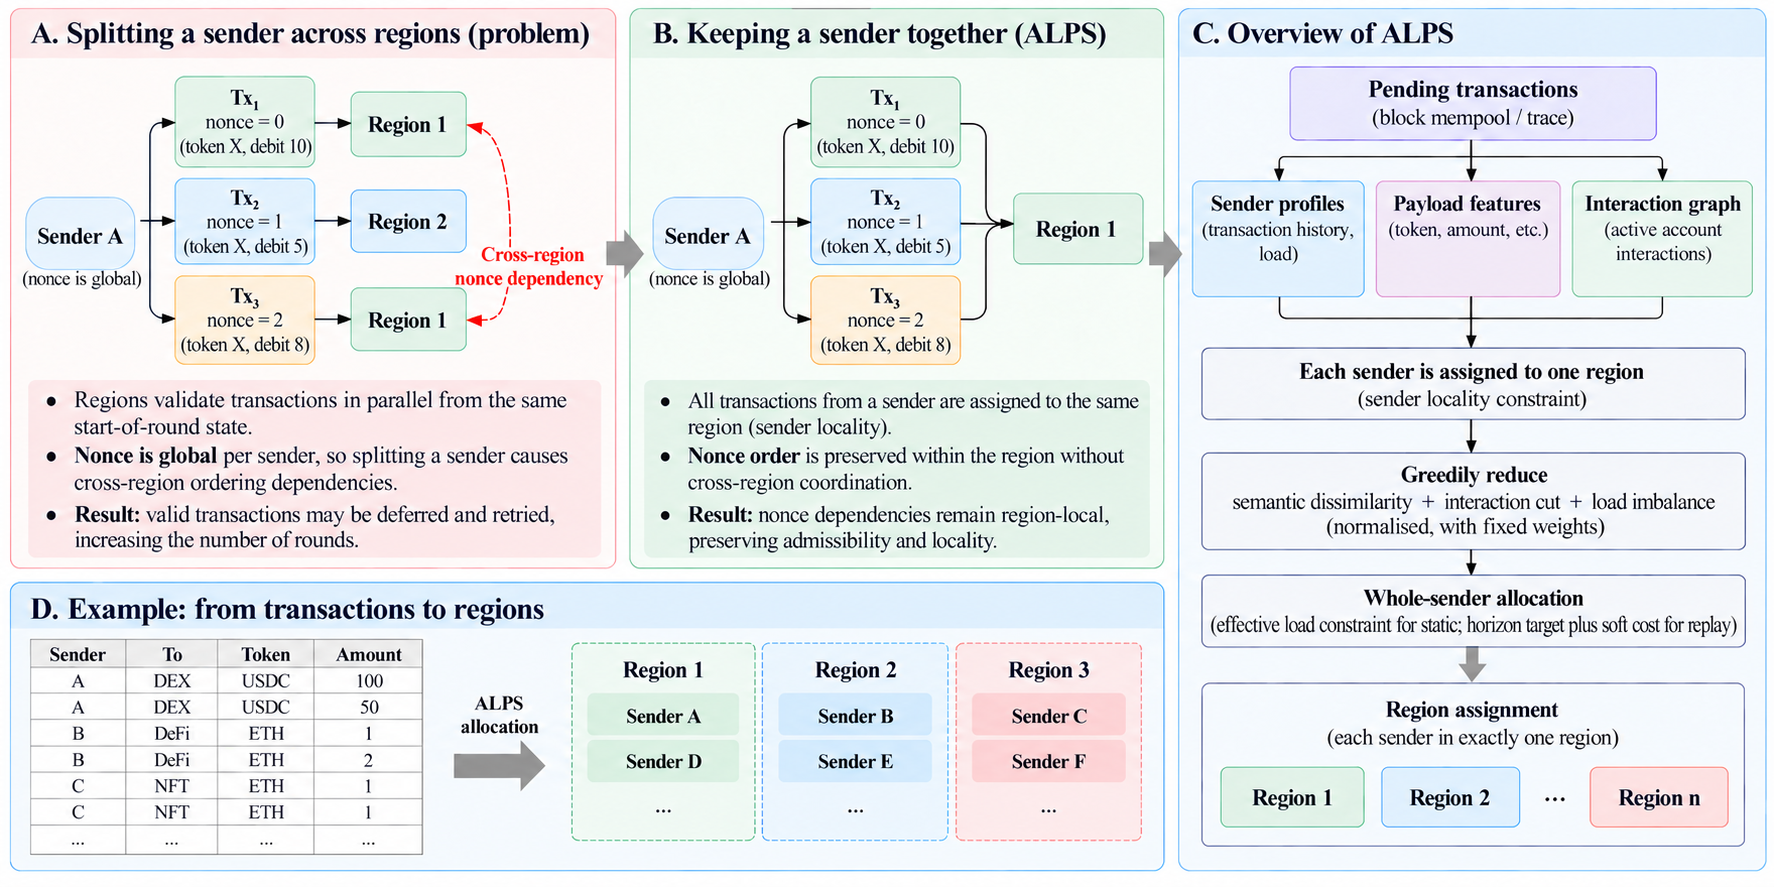
\includegraphics[width=\textwidth]{figures/pipeline-v2.png}
    \caption{Overview of ALPS and the role of sender locality. Splitting a sender
    across regions creates cross-region nonce dependencies under independent-barrier
    execution, whereas sender-local allocation preserves nonce order within a region.
    ALPS enforces whole-sender allocation and jointly optimises semantic locality,
    interaction cut, and historical-load balance under an effective load bound.}
    \label{fig:alps-overview}
\end{figure*}

\subsection{Proposed Method: ALPS}
\label{sec:alps}

ALPS uses sender-indivisible allocation and combines semantic locality,
interaction locality, and load control~(Figure~\ref{fig:alps-overview}).
The proposed method first performs static allocation and then extends it with
chronological sender pinning.

\subsubsection{Allocation Unit and Objective}

ALPS treats each active sender $a$ and its complete transaction sequence as one
indivisible unit. Let $w_a$ denote its historical transaction count, $x_a$ its
mean payload feature vector, and $e_{ab}$ the symmetrized number of observed
submitted calls in either direction between active senders $a$ and $b$. Define $W=\sum_a w_a$,
$M=\sum_{\{a,b\}}e_{ab}$, the mean regional load $\bar L=W/n$, and
$L_r=\sum_{a:z_a=r}w_a$. The exact dimensionless objective is

\begin{equation}
\label{eq:objective}
\begin{aligned}
J={}&\frac{1}{W}\sum_a w_a
 \frac{\lVert x_a-\mu_{z_a}\rVert_2^2}{s}\\
 &+\frac{\lambda_g}{M}\sum_{\{a,b\}}e_{ab}\mathbf{1}[z_a\ne z_b]\\
 &+\frac{\lambda_l}{n}\sum_{r=1}^{n}\left(\frac{L_r}{\bar L}\right)^2
\end{aligned}
\end{equation}

The heuristic greedily reduces this objective subject to one region per sender and
$L_r\leq C_{\mathrm{eff}}$. Because no feasible cap can be smaller than the
largest indivisible sender, the target cap is
$C_0=\max(\alpha\bar L,\max_a w_a)$. When a whole-sender packing satisfies $C_0$, ALPS sets
$C_{\mathrm{eff}}=C_0$; otherwise, the LPT fallback supplies a feasible
certificate and $C_{\mathrm{eff}}$ is relaxed only to the maximum load of that
certificate. In every reported run, $\max_a w_a\leq\alpha\bar L$ and no
packing relaxation was required, so $C_0=\alpha\bar L$ and
$C_{\mathrm{eff}}=C_0$. Here, $s$ is the median
nonzero semantic squared distance. The experiments use $\alpha=1.15$,
$\lambda_g=0.15$, and $\lambda_l=0.20$. Section~\ref{sec:results} reports the
graph-weight frontier rather than treating 0.15 as universally optimal.
The implementation requires $W>0$ and at least $n$ active senders, replaces
zero $M$ or $s$ by one, retains the preceding prototype for an empty region,
and resolves equal-cost choices by the smallest region index.

The preferred operating point depends on the deployment setting. Let $X$ be
the active-account interaction cut defined in Section~\ref{sec:method}. For a
deployment score $D_\kappa=R_{90}+\kappa X$, where $\kappa$ is the relative
penalty assigned to interaction-cut fraction in $R_{90}$-equivalent units,
ALPS is preferable to a baseline $B$ when

\begin{equation}
\label{eq:deployment}
\kappa > \kappa^\star=
\frac{R_{90}^{\textsc{alps}}-R_{90}^{B}}{X_B-X_{\textsc{alps}}}
\end{equation}

provided $X_{\textsc{alps}}<X_B$. A non-positive threshold means that ALPS
weakly dominates. This formulation makes the retrieval--interaction trade-off
explicit instead of hiding it inside a single composite score.

The three terms have different roles. The payload-distance term preserves
asset-query locality, the graph term reduces active-account cross-region
interactions, and the historical-load constraint limits how much of the trace
is assigned to one region. It is distinct from the per-round block capacity
$B$. Sender indivisibility is enforced outside the objective,
so optimisation cannot trade correctness for a lower objective value.

\begin{algorithm}[!t]
\caption{ALPS static allocation. Every operation moves a whole sender, so
sender locality is an invariant rather than a penalty.}
\label{alg:alps}
\small
\begin{algorithmic}[1]
\REQUIRE history $T_h$; regions $n$; $\alpha,\lambda_g,\lambda_l$
\ENSURE one pinned region $z_a$ per active sender
\STATE compute $(w_a,x_a)$ for active senders and graph weights $e_{ab}$
\STATE initialise $L_r\leftarrow0$ for every region; $z\leftarrow\emptyset$
\STATE $C_0 \leftarrow \max(\alpha\bar{L},\max_a w_a)$
  \COMMENT{target and indivisibility lower bound}
\STATE initialise $\mu_1,\ldots,\mu_n$ by transaction-weighted $k$-means
\FOR{senders $a$ in non-increasing $w_a$}
  \STATE $F \leftarrow \{r : L_r + w_a \le C_0\}$, or
  $\{\arg\min_r L_r\}$ if empty
  \STATE $z_a \leftarrow \arg\min_{r \in F} \Delta J(a \rightarrow r)$;
  $L_{z_a} \mathrel{+}= w_a$
\ENDFOR
\IF{$\max_r L_r > C_0$}
  \STATE reseed by LPT packing and recompute $L$
  \COMMENT{feasible certificate}
\ENDIF
\STATE $C_{\mathrm{eff}} \leftarrow \max(C_0,\max_r L_r)$
\REPEAT
  \STATE recompute weighted prototypes $\mu_r$
  \FOR{senders $a$ in non-increasing $w_a$}
    \STATE $r^\star \leftarrow \arg\min_r \Delta J(a:z_a\rightarrow r)$ s.t.
    $L_r+w_a\le C_{\mathrm{eff}}$
    \STATE move all of $a$ to $r^\star$ and update $L$ if $\Delta J<0$
  \ENDFOR
\UNTIL{no move accepted or six sweeps}
\RETURN $\{z_a\}$
\end{algorithmic}
\end{algorithm}

After transaction-weighted $k$-means initialisation, the implementation assigns
heavy senders first and then performs deterministic coordinate refinement with
prototype updates (Algorithm~\ref{alg:alps}). If the cost-aware seed violates
the target cap $C_0$, largest-processing-time-first (LPT) packing provides a
feasible whole-sender certificate. The refinement stage then enforces the
resulting $C_{\mathrm{eff}}$ as a hard constraint. No reported run required
relaxation beyond $C_0$. The implementation and fixed parameters are included
with the artifact.
Thus ALPS is a greedy local-search heuristic, not a global optimiser;
Proposition~1 establishes feasibility and monotone descent only.

\paragraph{Static Time Complexity}
Let $N=|T_h|$, $A$ be the active senders, $E$ their interaction edges, $I$ the
weighted $k$-means iterations, and $S\leq6$ the refinement sweeps. Profiling
costs $O(Nd)$, weighted $k$-means $O(InAd)$, sender sorting $O(A\log A)$, and
the seed or one sweep $O(n(Ad+E))$. Thus worst-case static time is
\begin{equation}
\label{eq:static_complexity}
O\!\left(Nd + InAd + A\log A + (S+1)n(Ad+E)\right).
\end{equation}
LPT adds $O(A\log A+A\log n)$ if invoked; no reported run required it.
Allocator storage excluding the input is $O(Ad+E+n)$.

\begin{proposition}[Monotone Constrained Refinement]
With fixed prototypes, every accepted ALPS move strictly decreases
\eqref{eq:objective} while preserving sender locality and the effective
capacity constraint. Replacing each prototype by its transaction-weighted mean
cannot increase the semantic term.
\end{proposition}

\begin{proof}
For each candidate move, ALPS evaluates the exact change in the sender's
semantic term, its incident interaction-cut edges, and the load terms of the
two affected regions. A move is accepted only when the total change is negative
and the destination region has sufficient remaining capacity. Because the
whole sender moves as one unit, sender locality is preserved. For fixed
assignments, the transaction-weighted mean minimises the within-region squared
semantic distance. Therefore, accepted moves strictly decrease the objective,
while prototype updates cannot increase its semantic term. Since the assignment
space is finite, unrestricted refinement reaches a one-move local optimum. The
implementation stops after at most six sweeps, so it may stop earlier while
still preserving monotonicity and feasibility.
\end{proof}

\subsubsection{Fixed-Horizon Chronological Placement}

A chronological allocator cannot build a sender profile from transactions that
have not yet occurred. The temporal version therefore learns prototypes and
assignments only from a chronological prefix. A known sender keeps its assigned
region. A sender absent from the history is assigned exactly once, when its
first future transaction arrives. The assignment uses the transaction's visible
payload, the receiver's region when the receiver is already placed, and the
current future-prefix load. The selected region is then pinned.

\begin{algorithm}[!t]
\caption{ALPS fixed-horizon chronological placement. A sender is assigned once, at its first
appearance, so later actions do not affect the earlier assignment.}
\label{alg:online}
\small
\begin{algorithmic}[1]
\REQUIRE history state $\{z_a\},\{\mu_r\}$; regions $n$; stream $T_f$;
predefined horizon $H_f$; $\alpha,\lambda_g,\lambda_l$
\ENSURE a pinned region for every sender in $T_f$
\STATE $C_f\leftarrow\alpha H_f/n$; initialise future loads $L_r\leftarrow0$
\FOR{transactions $t \in T_f$ in chronological order}
  \STATE $a \leftarrow \mathrm{sender}(t)$
  \IF{$a$ already has a region}
    \STATE keep $z_a$ unchanged \COMMENT{pinned; never revised}
  \ELSE
    \STATE $\rho \leftarrow$ region of $\mathrm{receiver}(t)$ if placed,
    else $\bot$
    \STATE $F\leftarrow\{r:L_r+1\leq C_f\}$, or all regions if empty
    \STATE $s_t\leftarrow$ median nonzero value in
    $\{\|\mathrm{feat}(t)-\mu_r\|^2:r=1,\ldots,n\}$, or $1$ if none
    \STATE $z_a \leftarrow \arg\min_{r\in F}
    [\,\|\mathrm{feat}(t)-\mu_r\|^2/s_t
    + \lambda_g \mathbf{1}[r \neq \rho]
    + \lambda_l {(L_r/C_f)}^2]$
    \STATE pin $z_a$
  \ENDIF
  \STATE route $t$ to $z_a$; $L_{z_a} \leftarrow L_{z_a}+1$
\ENDFOR
\end{algorithmic}
\end{algorithm}

Algorithm~\ref{alg:online} is a fixed-horizon chronological replay, not a fully
online deployment experiment: it predefines $H_f=|T_f|$ for each evaluation
suffix. Conditional on that horizon and the offline feature scaling described
in Section~\ref{sec:setup}, each placement uses only the prefix observed so far.
Later transactions do not affect earlier sender assignments. Here, $L_r$ counts
transactions observed so far and $C_f=\alpha H_f/n$ is the horizon target. When an unseen sender first appears, regions
that can accept that transaction without crossing $C_f$ form the candidate set;
if none remain, all regions are considered. The load term then acts as a soft
cost within that set. This admission test applies only when a sender is first
pinned: later activity from that sender must follow its pinned region and can
therefore drive realised load above $C_f$. Thus, unlike the static allocator,
the chronological rule provides no lifetime hard-cap guarantee. Sender locality remains
structural while activity drift can exceed the $1.15$ horizon target.

\paragraph{Chronological Time Complexity}
With a hash-map assignment table, routing a transaction from an already pinned
sender takes $O(1)$ expected time. A previously unseen sender is placed only
once; evaluating its semantic and load-aware cost over all $n$ regions costs
$O(nd)$. Therefore, for a future stream of $F$ transactions containing $U$
previously unseen senders, chronological placement costs
\begin{equation}
\label{eq:online_complexity}
O(F+Und),
\end{equation}
with the more expensive $O(nd)$ decision paid only at each sender's first
appearance. The assignment map grows by $O(U)$ entries over the future stream.

This temporal split is used as a robustness check rather than a methodological
novelty claim. A-TxAllo also uses a chronological 9:1 partition, carries the
previous allocation forward, and explicitly places new nodes using newly
committed transactions~\cite{txallo2023}. The evaluation in this paper instead
uses four fixed history horizons, pins each sender at its first appearance, and
evaluates retrieval together with interaction cut and load.
For fairness, every fixed-horizon replay baseline carries its history assignment
forward and assigns each unseen sender once using that baseline's rule; the
assignment is then pinned. The replay allocator is a related heuristic rather than the
static graph objective: its graph term is replaced by one currently placed
receiver indicator.

\section{Experimental Setup}
\label{sec:setup}
\label{sec:method}

This section describes the traces and feature construction, the compared
schemes and execution settings, and the evaluation metrics and chronological
protocol.

\subsection{Traces and Feature Construction}

Table~\ref{tab:data} summarises three Ethereum mainnet traces covering eight
ERC-20 contracts and one held-out BNB Smart Chain (BSC) trace with a disjoint set of
eight tokens. D1--D3 include only direct
\texttt{transfer(address,uint256)} calls. Therefore, the outer signer is both
the debited token owner and the actual account-nonce owner. Observed signer
nonces are rank-normalised per sender without changing their relative order.
Because other account transactions are absent, this models the collected
direct-transfer stream, not the complete Ethereum mempool. The traces cover
non-overlapping spans on 14, 13, and 7 August 2026, with D3 separated from the
others by one week. D1 contains documented collection gaps, while D2, D3, and
C1 scan their full stated spans.

Selector, calldata, and nonce semantics are common to both chains. C1 is
challenging for semantic placement because one
token accounts for $94.9\%$ of submitted calls, compared with
$69.7$--$72.7\%$ on Ethereum. A secondary \texttt{Transfer}-log trace extends
the balance-locality population but cannot identify outer signers for
router-mediated calls. It is therefore excluded from nonce-related claims.
Artifact manifests provide block ranges, chain IDs, contract addresses,
filters, hashes, RPC endpoints, and provenance.

\begin{table}[t]
\caption{Measured traces. Blocks/span shows represented blocks over the inclusive
height span. D1 has documented gaps; D2, D3, and C1 cover their full spans.
Top token is the share of the most frequent contract; Multi-tok. is the share
of calls/events from repeat senders active in multiple tokens.}
\label{tab:data}
\centering
\small
\resizebox{\columnwidth}{!}{%
\begin{tabular}{llrrrrr}
\toprule
Trace & Chain & Calls/events & Blocks/span & Senders & Top token & Multi-tok.\\
\midrule
Direct calls (D1) & ETH & 34,326 & 513/714 & 18,747 & 69.7\% & 19.5\%\\
Prior-day (D2) & ETH & 39,425 & 713/714 & 20,719 & 70.0\% & 20.9\%\\
Prior-week (D3) & ETH & 45,893 & 499/500 & 27,963 & 72.7\% & 19.9\%\\
Cross-chain (C1) & BSC & 25,728 & 2489/2500 & 14,082 & 94.9\% & 10.3\%\\
Transfer logs & ETH & 17,445 & 81/137 & 7,195 & --- & ---\\
\bottomrule
\end{tabular}}
\end{table}

Collection uses public JSON-RPC endpoints. Complete-scan collectors retain
transaction hashes and stop if a block is missing. Eleven self-transfers are
excluded from the log trace, leaving 17,445 evaluated events in
Table~\ref{tab:data}. Direct-call collection requires a listed token target,
the standard selector, nonzero decodable calldata, and a non-self recipient;
router/proxy calls are excluded and duplicate sender nonces are removed during
loading. Receipts were not queried, so submitted calls that later reverted are
not distinguished. Accordingly, D1--D3 and C1 are submitted direct-call
workloads, and ``call'' does not assert a successful token state transition;
reverted submissions may still consume a nonce and influence locality metrics.

Raw ERC-20 values are not directly comparable across token decimals and price
scales. For each token, the raw value is divided by its trace median, clipped to
$[0.1,20]$, and used in the balance stress model. Clustering features combine a
scaled exact token one-hot vector with
$\log(1+\mathrm{relativeAmount})$. No Gaussian jitter or synthetic clustering
coordinate is used. Therefore, when transaction $k$-means splits a dominant
token, the split is based on an observed amount difference.
Token medians are fixed offline from each complete trace, including in the
fixed-horizon replay, so feature scaling uses suffix information. Sender profiles,
prototypes, and assignments use only the history prefix, but the preprocessing
scale is not a strictly online estimate. A production streaming allocator would
require online feature-statistic maintenance.

\subsection{Schemes and Execution}

\begin{table}[t]
\caption{Design properties of the compared methods. Local denotes
sender/guarded-state locality; Cap denotes a hard static historical-load constraint;
Coord denotes coordination beyond the independent barrier.}
\label{tab:design}
\centering
\small
\setlength{\tabcolsep}{3pt}
\begin{tabular}{@{}lccccc@{}}
\toprule
Method & Local & Sem. & Cut & Cap & Coord.\\
\midrule
ADDR-MOD      & Yes & No  & No  & No  & No\\
TX-KMEANS     & No  & Yes & No  & No  & Retry\\
SENDER-KMEANS & Yes & Yes & No  & No  & No\\
S-KM-BAL      & Yes & Yes & No  & Yes & No\\
METIS         & Yes & No  & Yes & No  & No\\
TXALLO        & Yes & No  & Yes & No  & Protocol\\
ALPS          & Yes & Yes & Yes & Yes & No\\
\bottomrule
\end{tabular}
\end{table}

The main static evaluation compares all methods except METIS and TXALLO. ADDR-MOD uses
$a\bmod n$, TX-KMEANS clusters individual transactions, and the sender-based
variants cluster mean features of active senders. S-KM-BAL additionally uses
the $1.15\times$ historical-load target, while ALPS uses the joint objective described in
Section~\ref{sec:alps}. Section~\ref{sec:txallo} separately compares METIS and TXALLO.

The evaluation varies $n\in\{2,3,4,6,8,11\}$ with a regional block capacity of
250. For the global nonce experiment, each (account, token) debit key is funded
with its complete observed outgoing amount plus a cushion of one normalised
balance unit. Therefore, both
sequential execution and any correct retrying schedule can commit the full
trace. Extra rounds reflect ordering and partitioning effects rather than
arbitrary balance failures. Each regional mempool selects currently ready
sender/nonce entries, commits up to capacity, retains future-nonce
transactions, and retries them after the barrier.

The complete static sweep uses deterministic seed 0 with $k$-means
\texttt{n\_init=10}. The temporal, frontier/ablation, and TxAllo comparisons use
three initialisations. Allocation-sensitive conclusions are therefore reported
from these sensitivity runs as well as the exact static audit.
The capacity and allocator-runtime audits use five fresh initialisations.

For the balance-safety experiment, each observed (account, token) key instead
receives the same stress balance, varied over
$\{1000,600,400,250,150,100,60\}$. Account nonces are ignored only in this
experiment to expose simultaneous guarded-key debits. A negative balance after
the synthetic additive merge is an exact balance-safety witness for that run,
not a reconstruction of historical execution; token balances are never pooled
across contracts.

State and scheduling experiments set proof-of-work difficulty to zero. The
evaluation reports barrier rounds and the schedule-level commit rate,
$Q_s=N_c/R$, where $N_c$ is the number of committed transactions and $R$ is the
number of rounds. This is not machine-dependent wall-clock TPS. With regional
capacity $B$, $Q_s/(nB)$ represents schedule utilisation and isolates dependency
stalls from hashing, storage, networking, and consensus. The simulator retains
a genuine SHA-256 path for separate benchmarking, but no wall-clock claim
depends on it.

\subsection{Metrics and Temporal Protocol}

The evaluation reports split senders and guarded keys, transactions issued by
split senders, barrier rounds, deferred nonce checks, maximum-to-mean regional
load, and the active-account interaction cut. For a given allocation, let
$T_{\mathrm{act}}$ be submitted calls whose receiver also appears as an active sender.
The interaction cut is
\[
X=\frac{|\{t\in T_{\mathrm{act}}:z_{\mathrm{sender}(t)}\neq
z_{\mathrm{receiver}(t)}\}|}{|T_{\mathrm{act}}|},
\]
and interaction coverage is $|T_{\mathrm{act}}|/|T|$. Receiver-only addresses
are therefore excluded from the cut rather than automatically counted as
cross-region. Regional load is reported as $\max_r L_r/\bar L$. For semantic
retrieval locality, regions are ranked for each token by that token's call/event
count; $R_{90}$ is the number of highest-ranked regions required to cover at
least 90\% of that token's calls/events, averaged over the evaluated tokens. Thus,
lower $R_{90}$ means fewer regions need to be scanned, not lower measured query
latency.

Static interaction coverage depends only on the trace and is therefore
strategy-invariant: $53.8\%$ for D1, $56.6\%$ for D2, $60.6\%$ for D3, and
$45.7\%$ for C1. This conditional metric matches ALPS's active-sender graph
while keeping the denominator explicit.

The fixed-horizon chronological replay uses $n=6$, history fractions
$\{0.5,0.6,0.7,0.8\}$, and three $k$-means initialisations, giving 12
history/future configurations per method. Figures report the mean and standard
deviation across these configurations as sensitivity summaries rather than as
independent repeated chain samples. Across the four traces, 60.0\% of future
transactions come from senders absent from the training prefix, making
cold-start handling important.

\section{Performance Evaluation}
\label{sec:results}

The evaluation examines safety, retry cost, locality, temporal robustness,
component effects, and comparison with TxAllo. The headline parameters use
$\lambda_g=0.15$ and $\alpha=1.15$, selected using D1 as the development trace
and then held fixed; D2, D3, and C1 provide parameter-holdout checks on
temporally distinct traces. Each static allocation is nevertheless fitted and
scored on the same trace, so these are not out-of-sample allocation tests.
The static and head-to-head evaluations cover all six region counts, while the
stress, temporal, and mechanism analyses use $n=6$. The operating frontier
varies only $\lambda_g$, and each ablation removes one component at a time.
Overall, the static sweep contains 120 trace/region/scheme measurements, and the
balance-stress experiment contains 175 measurements (140 sender-local and 35
TX-KMEANS).

\subsection{Admissibility under Payload Partitioning}

TX-KMEANS violates sender locality on every trace and, at larger region
counts, also violates guarded-key locality. Across the 96 sender-local
measurements---ADDR-MOD, both sender $k$-means variants, and ALPS over four
traces and six region counts---the number of split guarded keys, split senders,
and overdrawn accounts is exactly zero, and every execution commits the complete
trace. In contrast, TX-KMEANS splits 66--1{,}592 senders and up to 1{,}334
guarded keys. Across the four traces and region counts, transactions issued by
split senders account for $10.3$--$44.4\%$ of the corresponding trace
(Fig.~\ref{fig:sweep}(a)). Table~\ref{tab:headline} reports the detailed results
for $n=6$.

The distinction between guarded-key locality and sender locality is clear at
$n=2$. Across all four traces, TX-KMEANS splits no guarded keys but still splits
66--551 senders. With two regions, clustering places complete token populations
on each side, so every $(\text{account},\text{token})$ balance remains
region-local and balance safety is preserved. However, accounts that transact
across multiple tokens can still be divided between regions, creating
cross-region dependencies for the account-wide nonce. This result directly
shows the difference between guarded-key locality and sender locality and is
visible because balances are modelled separately for each token.

The balance-stress experiment further confirms this behaviour. Across 175
measurements---five traces, seven starting balances, and five schemes---TX-KMEANS
overdraws 6--48 unique accounts in each of its 35 rows, while all 140 sender-local rows
record zero overdraws. The lowest-balance tail is non-monotone because tighter
balances can cause regional transfers to fail before two conflicting debits are
both accepted and merged. Therefore, the number of witnesses is not expected
to increase monotonically.

\begin{table}[t]
\caption{Results at $n=6$ for all direct-call traces. Split keys are guarded
$(\text{account},\text{token})$ keys. An overdrawn account is a unique account
with at least one negative guarded key; ranges span the seven-level balance
stress. Lower is better except $Q_s$.}
\label{tab:headline}
\centering
\scriptsize
\setlength{\tabcolsep}{2pt}
\begin{tabular}{@{}lrrrrrrr@{}}
\toprule
Method & Split & Rounds & $Q_s$ & Overdrawn & $R_{90}$ & Load & Active cut\\
 & keys & & & accts. & & & (fraction)\\
\midrule
\multicolumn{8}{@{}l}{D1 ETH 08-14}\\
\quad ADDR-MOD & 0 & 33 & 1,040 & 0 & 5.88 & 1.43 & .837\\
\quad TX-KMEANS & 1,021 & 1,068 & 32 & 19--48 & 1.38 & 2.27 & .425\\
\quad S-KM-BAL & 0 & 27 & 1,271 & 0 & 2.25 & 1.15 & .646\\
\quad ALPS & 0 & 27 & 1,271 & 0 & 3.00 & 1.15 & .260\\
\addlinespace
\multicolumn{8}{@{}l}{D2 ETH 08-13}\\
\quad ADDR-MOD & 0 & 37 & 1,066 & 0 & 5.88 & 1.39 & .841\\
\quad TX-KMEANS & 1,061 & 1,388 & 28 & 20--48 & 1.38 & 2.28 & .432\\
\quad S-KM-BAL & 0 & 31 & 1,272 & 0 & 2.38 & 1.15 & .670\\
\quad ALPS & 0 & 31 & 1,272 & 0 & 2.88 & 1.15 & .279\\
\addlinespace
\multicolumn{8}{@{}l}{D3 ETH 08-07}\\
\quad ADDR-MOD & 0 & 38 & 1,208 & 0 & 5.50 & 1.22 & .834\\
\quad TX-KMEANS & 1,067 & 843 & 54 & 12--36 & 1.38 & 2.08 & .614\\
\quad S-KM-BAL & 0 & 36 & 1,275 & 0 & 3.12 & 1.15 & .818\\
\quad ALPS & 0 & 36 & 1,275 & 0 & 2.88 & 1.15 & .528\\
\addlinespace
\multicolumn{8}{@{}l}{C1 BSC}\\
\quad ADDR-MOD & 0 & 21 & 1,225 & 0 & 4.62 & 1.21 & .837\\
\quad TX-KMEANS & 478 & 448 & 57 & 13--34 & 1.25 & 2.93 & .413\\
\quad S-KM-BAL & 0 & 20 & 1,286 & 0 & 2.62 & 1.15 & .859\\
\quad ALPS & 0 & 19 & 1,354 & 0 & 2.00 & 1.07 & .236\\
\bottomrule
\end{tabular}
\end{table}

\subsection{Retry Cost of Sender Fragmentation}

Deferring and retrying future-nonce transactions restores eventual commit, but
it does not remove the scheduling cost. Every scheme commits $100\%$ of every
trace with no pending transactions once future nonces are retried. However,
TX-KMEANS requires 156--1{,}760 rounds, compared with 11--106 for ALPS, and
performs up to $3.13$ million future-nonce checks. Its schedule-level commit rate,
$Q_s$, falls to 22--253 committed transactions per round, compared with
432--2{,}338 for ALPS.

At $n=6$, ALPS achieves approximately $40\times$, $45\times$, $24\times$,
and $24\times$ higher schedule-level commit rate than TX-KMEANS on D1, D2, D3,
and C1, respectively (Fig.~\ref{fig:sweep}(b), Table~\ref{tab:headline}).
The reason is that preserving the account-wide nonce order for fragmented
senders forces progress to continue across barriers, creating a strong
scheduling penalty on every trace.

\begin{figure*}[t]
\centering
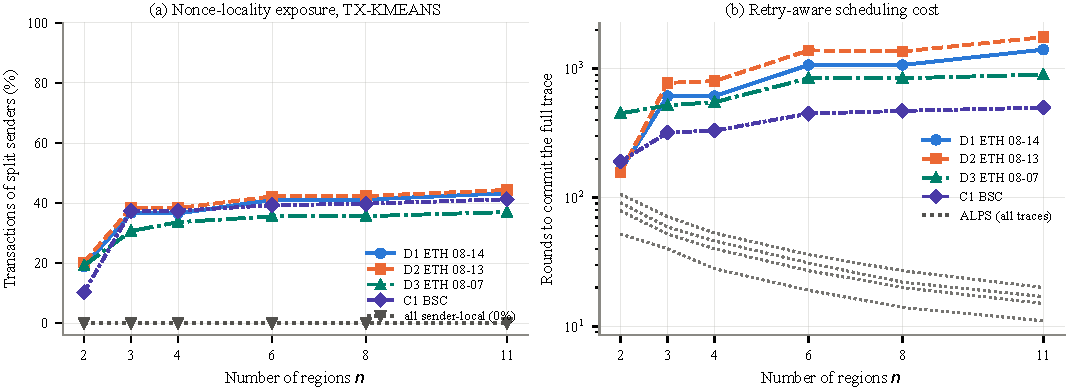
\includegraphics[width=.66\textwidth]{figures/fig_sweep.pdf}
\caption{Locality violations and retry-aware scheduling cost across the four
direct-call traces. Sender-local schemes have zero split-sender exposure in
(a), while (b) compares TX-KMEANS and ALPS round counts.}
\label{fig:sweep}
\end{figure*}

\subsection{Locality and Load Trade-offs}

Relative to ADDR-MOD, enforcing sender locality does not prevent ALPS from
improving both locality metrics on these traces; the additional cost is allocator
computation (Section~\ref{sec:components}). ALPS improves both locality metrics
over ADDR-MOD in all 24 trace/region settings. $R_{90}$ decreases by
$18.8$--$68.5\%$ (mean $45.9\%$), while the interaction cut decreases by
$35.2$--$75.9\%$ (mean $57.7\%$), with static load never exceeding the $1.15$
target.

A more informative comparison is with balanced sender $k$-means, which is
already admissible. ALPS reduces the interaction cut in all 24 settings by
$12.8$--$82.5\%$ (mean $50.9\%$). It also improves $R_{90}$ in 19 settings,
ties in two, and regresses in three. These three retrieval-locality trade-offs
occur at $n=6$ on D1 and D2 and at $n=4$ on D3; only the D1 case is on the
development trace used for parameter selection. We therefore report these
exceptions explicitly rather than claiming universal dominance. In most
settings, ALPS provides a strict improvement; otherwise, the break-even ratio
$\kappa^\star$ identifies when the simpler scheme is preferable under the score
in~\eqref{eq:deployment}. For the D1 $n=6$ setting, $\kappa^\star=1.94$:
weights above this value favour ALPS because they place greater relative
penalty on interaction cut, whereas smaller weights favour SENDER-KMEANS-BAL.
At higher region counts, ALPS often weakly dominates, making the threshold
non-positive.

Figure~\ref{fig:locality} shows why these exceptions are limited to small $n$.
The retrieval cost of ADDR-MOD increases sharply with the number of regions,
giving semantic partitioning more room for improvement. At $n=11$, ALPS
improves $R_{90}$ over balanced sender $k$-means by $10.0$--$37.8\%$ across
all four traces. Unconstrained SENDER-KMEANS achieves strong semantic locality
but becomes highly imbalanced, reaching a load of $4.45$ at $n=11$. In
contrast, the capacity-aware schemes never exceed $1.15$.

\begin{figure*}[t]
\centering
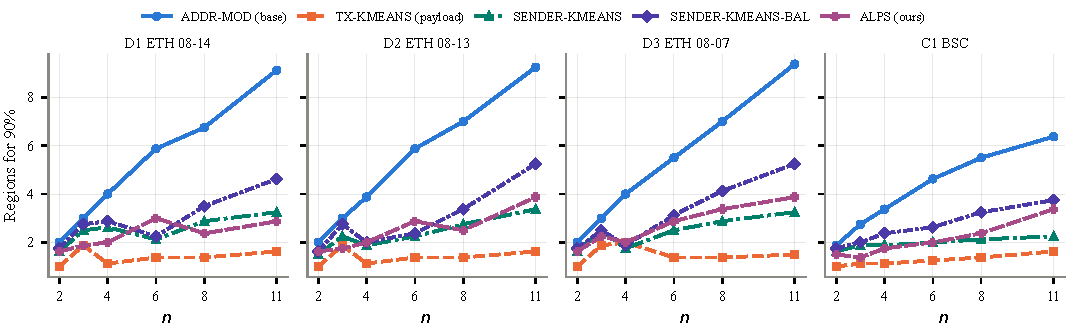
\includegraphics[width=.66\textwidth]{figures/fig_locality.pdf}
\caption{Semantic retrieval cost across all direct-call traces. TX-KMEANS is an
infeasible, capacity-unconstrained comparator that violates sender locality;
the other methods are sender-local.}
\label{fig:locality}
\end{figure*}

\subsection{Fixed-Horizon Replay Robustness}

The fixed-horizon replay preserves sender locality by construction because each
unseen sender is assigned once and pinned; it is an invariant, not a
differentiating chronological-performance metric.

Compared with balanced sender $k$-means, ALPS reduces the conditional future
interaction cut among transactions whose receiver is already placed by
$19.3\%$, $23.7\%$, $37.9\%$, and $14.1\%$ on D1, D2, D3, and C1,
respectively, while also lowering the observed load
(Fig.~\ref{fig:temporal}). Retrieval shows a mixed result: $R_{90}$ is
$4.8\%$ and $8.0\%$ higher on D1 and D2, nearly unchanged on D3, and
$30.3\%$ lower on C1. Unconstrained SENDER-KMEANS achieves lower interaction
cuts on D3 and C1 ($.327$ and $.576$, compared with $.513$ and $.745$ for
ALPS), but with much higher loads of $3.68$ and $2.58$, compared with $1.48$
and $1.43$ for ALPS.

C1 shows the weakest conditional interaction-cut improvement. ALPS improves over hashing by
$11.9\%$ on C1, compared with $28.8$--$38.7\%$ on the Ethereum traces. One
token accounts for $94.9\%$ of C1 submitted calls, and $62.2\%$ of future traffic
comes from unseen senders. As a result, first-transaction payloads provide
limited information for distinguishing accounts. Sender pinning still preserves
safety. The fixed-horizon allocator uses a $1.15$ target both to filter feasible
regions when a sender first appears and to scale its load cost, but it does not
impose a lifetime hard cap; pinned-sender activity can therefore drive observed
future load above $1.15$.

The causal interaction cut includes only receiver placements available at the
time of arrival, giving coverage of $26.4$--$44.3\%$ across the traces.
Unplaced receivers are reported separately. Overall, $60.0\%$ of future traffic
comes from unseen senders, which explains much of the gap between static and
chronological performance.

\begin{figure*}[t]
\centering
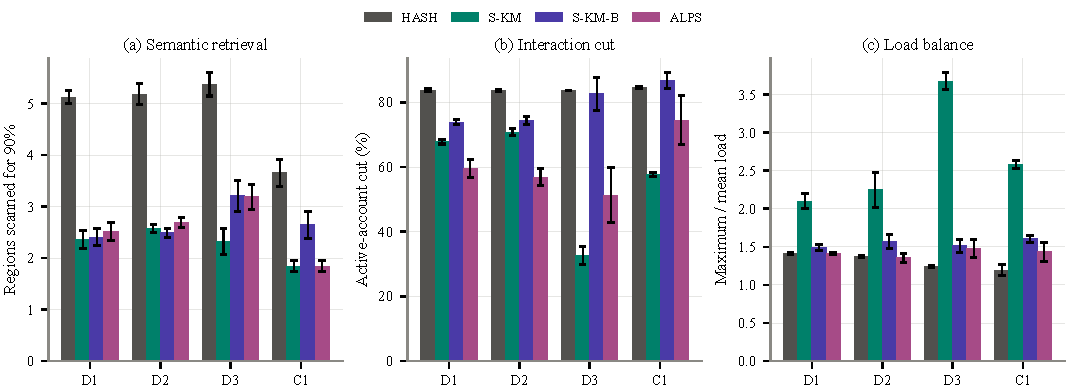
\includegraphics[width=.66\textwidth]{figures/fig_temporal.pdf}
\caption{Fixed-horizon chronological replay at $n=6$. Bars show means over four history
fractions and three initialisations; error bars show standard deviations. S-KM
and S-KM-B denote sender $k$-means and its balanced variant.}
\label{fig:temporal}
\end{figure*}

\subsection{Component Analysis and Allocator Overhead}
\label{sec:components}

The same component effects appear across all four traces. Removing the semantic
term degrades retrieval locality: $R_{90}$ is $5.00$, $5.25$, $4.88$, and
$4.12$ on D1, D2, D3, and C1, respectively, versus address hashing's $5.88$,
$5.88$, $5.50$, and $4.62$. The interaction cut decreases as expected.
Removing the capacity cap increases load to $1.28$--$1.52$, exceeding
the measured $1.15$ maximum-imbalance target. Setting $\lambda_g=0$ removes the
interaction term and produces a semantic-plus-load ALPS variant. This variant is
close to, but not identical to, balanced sender $k$-means because ALPS uses
transaction-weighted prototypes and exact objective refinement. Comparing it
with positive graph weights isolates the effect of the interaction term without
assuming algebraic equivalence to that baseline.

Figure~\ref{fig:frontier} shows the operating curve for each trace. The fixed
$\lambda_g=0.15$ lies in the low-cut region of every measured curve, although no
universal knee is claimed. C1 begins to flatten earlier than the three Ethereum
traces. Beyond $0.35$, the curve may flatten or reverse, which is consistent
with the non-convex discrete search.

A five-seed audit varies $\alpha\in\{1.05,1.10,1.15,1.25,1.50\}$ at six
regions on all four traces. No run relaxes its requested cap. Moving from 1.05
to 1.15 lowers cut on every trace; larger values give trace-dependent,
non-monotone changes. Error intervals in the artifact quantify initialisation,
not workload-sampling, variability.

Allocator overhead remains modest at the measured scale. On D1 prefixes of
5,000, 10,000, 20,000, and 34,326 calls, fresh single-worker runs over three
seeds require median profile-plus-allocation times of 2.50, 5.32, 8.08, and
12.60~s, respectively, on an Intel i9-14900. At the full trace, with 18,747
active senders and 16,120 interaction edges, the peak process working set is
248.4~MiB, and no run relaxes the capacity bound. These measurements represent
allocator overhead, not production TPS.

A separate five-seed, fresh-process comparison at six regions gives tracewise
median ranges of $<0.01$~s (ADDR-MOD), $0.16$--$0.26$~s (TX-KMEANS),
$0.29$--$0.68$~s (S-KM-BAL), $0.13$--$0.28$~s (METIS), $4.17$--$6.88$~s
(TxAllo), and $10.99$--$15.74$~s (ALPS). CSV loading is excluded; required
profile or graph construction is included.

\begin{figure}[t]
\centering
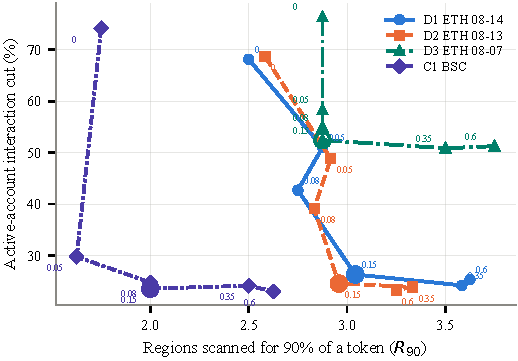
\includegraphics[width=.76\columnwidth]{figures/fig_frontier.pdf}
\caption{ALPS retrieval--interaction trade-off across all direct-call traces.
Point labels give $\lambda_g$ and the fixed $0.15$ point is circled; lower
values are better on both axes.}
\label{fig:frontier}
\end{figure}

\subsection{Comparison with Graph Partitioning and TxAllo}
\label{sec:txallo}

Sender-weighted METIS records zero splits in all 72 runs. Across all 24
trace/region settings, ALPS lowers its $R_{90}$ by 18.2--64.4\% (mean 39.4\%),
whereas METIS achieves a 32.9--91.1\% lower interaction cut than ALPS
(mean 63.4\%) and reaches a
maximum load of 1.058. Thus graph cut optimises interaction locality but does
not optimise semantic retrieval locality. This trade-off arises because METIS
operates on account-interaction topology, whereas $R_{90}$ depends on
token-specific retrieval concentration.

The closest algorithmic comparison is the TxAllo allocation objective~\cite{txallo2023}, which allocates
accounts using community detection and jointly optimises cross-shard traffic and
workload balance. This paper reimplements its allocation objective using Louvain
initialisation, candidate-community moves, and coordinate descent on its
throughput score. For shard $r$, the implementation forms workload $\sigma_r$
from local transaction count plus $(\eta-1)$ times each incident cross-shard
edge weight and greedily moves an account only to a neighbouring community's
shard when this strictly lowers $\max_r\sigma_r$; ties keep the current shard.
It uses $\eta=2$, at most eight sweeps, and stops when a sweep accepts no move.
Protocol components, including consensus, settlement,
brokers, and the A-TxAllo epoch update, are excluded because they change the
execution semantics. The comparison therefore evaluates allocation objectives
under the same execution model rather than deployed throughput, using $\eta=2$,
eight coordinate sweeps, and three-seed means over eight trace/region settings.

The reimplementation is account-keyed and records zero split senders and guarded keys in all
eight trace/region settings. Thus, this independently designed workload-aware
allocator also satisfies the locality requirement described in
Section~\ref{sec:model}. The two methods favour different objectives. Relative
to ALPS, the reimplemented objective reduces the active-account cut in all eight trace/region
settings by $13.5$--$79.2\%$ (mean $50.6\%$). In contrast, ALPS reduces
$R_{90}$ in all eight trace/region settings by $40.5$--$60.8\%$
(mean $47.3\%$). These results expose an objective trade-off: the reimplementation assigns
greater relative emphasis to active-account cross-region interaction, whereas
ALPS explicitly includes retrieval locality through $R_{90}$. At $n=11$,
the reimplementation also permits loads of $1.16$--$1.67$, whereas static ALPS maintains its
effective load constraint at or below $1.15$.

A one-factor sensitivity analysis at $n=6$ varies
$\eta\in\{1.25,1.5,2,3,4\}$ with eight sweeps and varies the sweep cap over
$\{4,8,16,32\}$ with $\eta=2$, across four traces and three seeds. ALPS retains
lower $R_{90}$ in all 12 trace/seed configurations for every value of $\eta$.
The reimplementation retains the lower interaction cut in all 12 trace/seed configurations
through $\eta=3$ and in 10 of 12 configurations at $\eta=4$. It exceeds the
$1.15$ load target once at each of $\eta=3$ and $\eta=4$. All four sweep caps
produce identical metrics, indicating convergence within four sweeps in these
settings.

\FloatBarrier

\section{Conclusion and Future Work}
Semantic partitioning is not only an optimisation problem; the allocation must also be executable. In the concurrent same-snapshot, additive-merge model, guarded-key locality is necessary and sufficient for balance non-negativity; this is not a theorem about full Ethereum validity or coordinated execution. Splitting a sender creates cross-region nonce-ordering dependencies, and ALPS enforces sender locality for the evaluated direct calls. Retry-aware transaction clustering eventually commits the observed nonce-ordered stream, but its 1,068 barrier rounds at six regions show that eventual commit need not be efficient. Static ALPS greedily reduces retrieval cost, conditional active-account interaction cut, and historical allocation load under a hard effective load constraint, equal to the $1.15$ target in every headline static run. The related fixed-horizon chronological replay preserves sender locality but uses offline feature scaling and has no lifetime load-cap guarantee. The evaluation is limited to short submitted-call workloads from two EVM chains; the Ethereum traces share a contract set, direct calls exclude routers and other nonce-consuming transactions, receipts and historical balances are not reconstructed, and trace-wide amount medians are fixed offline. The TxAllo result covers a reimplemented allocation objective, not its protocol. Finally, $R_{90}$ measures region scans rather than latency, and the round-based commit rate measures scheduling efficiency rather than production TPS. Future work will consider diverse traces, archive-state replay, general read/write sets, migration, and protocol integration.

\bibliographystyle{IEEEtran}
\newcommand{\BIBdecl}{\scriptsize}
\IEEEtriggeratref{6}
\bibliography{references}

\end{document}
